\begin{appendices}
\addtocontents{toc}{\protect\setcounter{tocdepth}{2}}\makeatletter
\addtocontents{toc}{%
  \begingroup
  \let\protect\l@chapter\protect\l@section
  \let\protect\l@section\protect\l@subsection
}
\makeatother



    





\begin{comment}
\section{Flowcharts}\label{app:flowcharts}

\begin{figure}[htp]
    \centering
    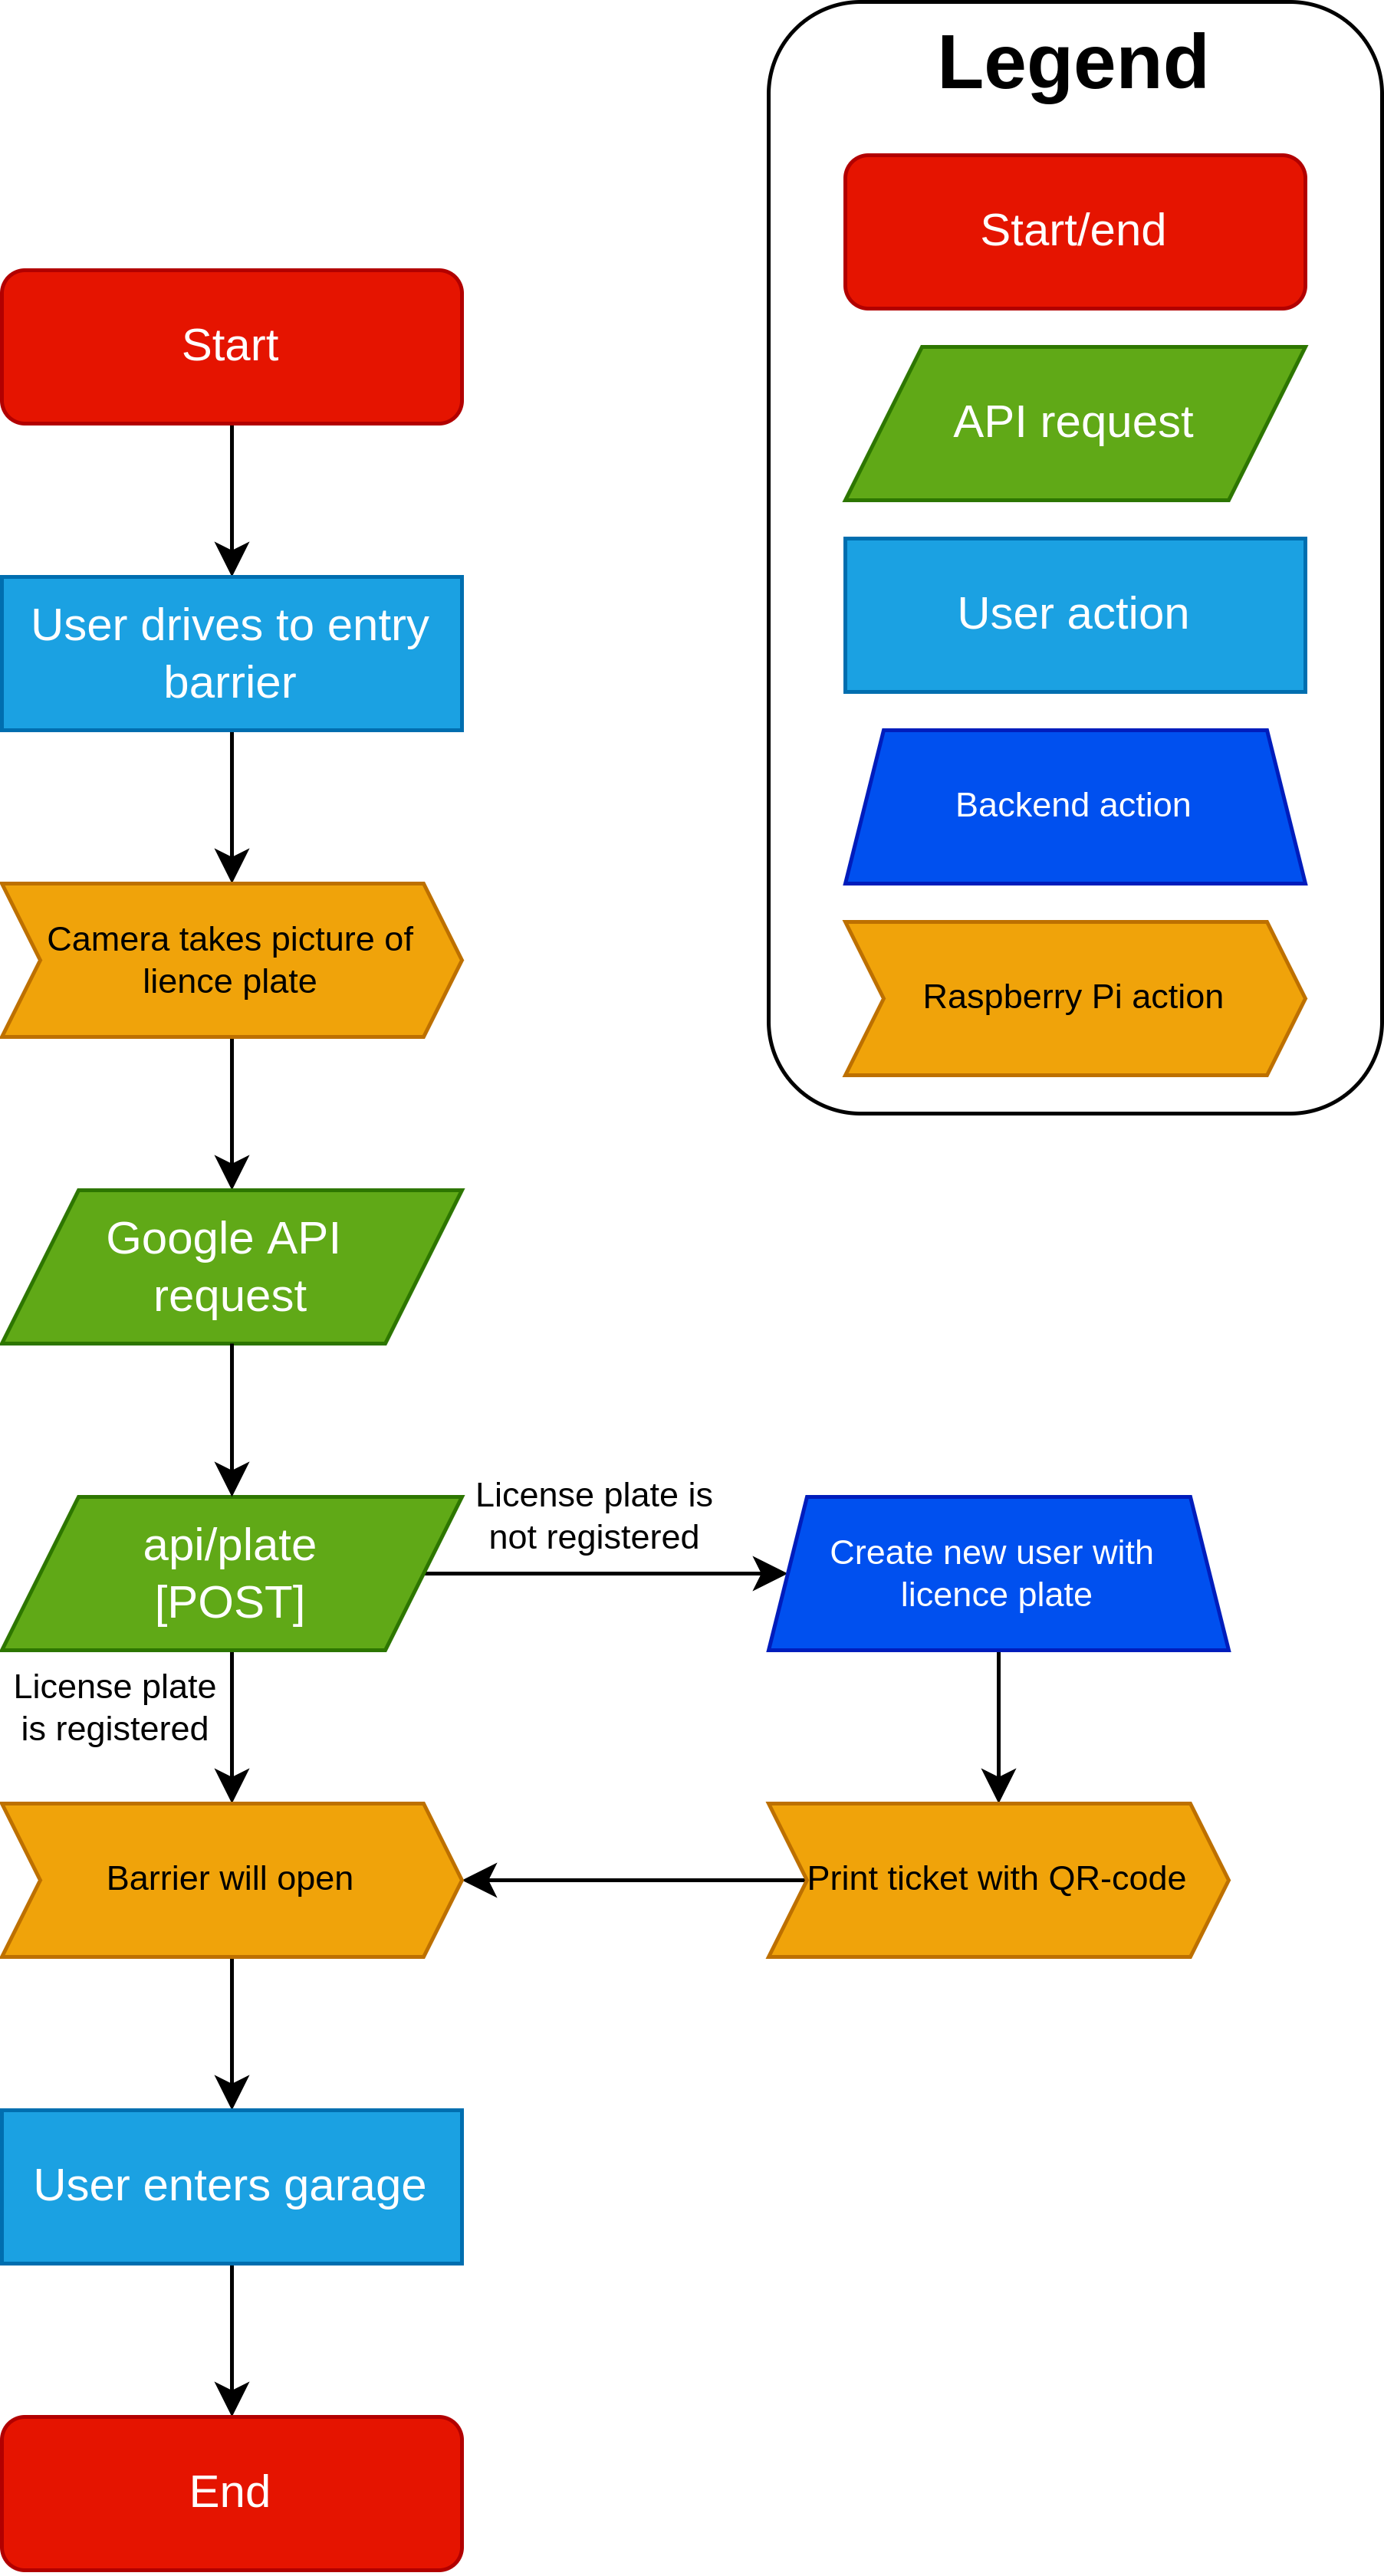
\includegraphics[width=7cm]{images/garage_enter.drawio.png}
    \caption{Flowchart of the entering process of the garage in both hardware, software and user terms.}
    \label{fig:garage-enter}
\end{figure}

\begin{figure}[htp]
    \centering
    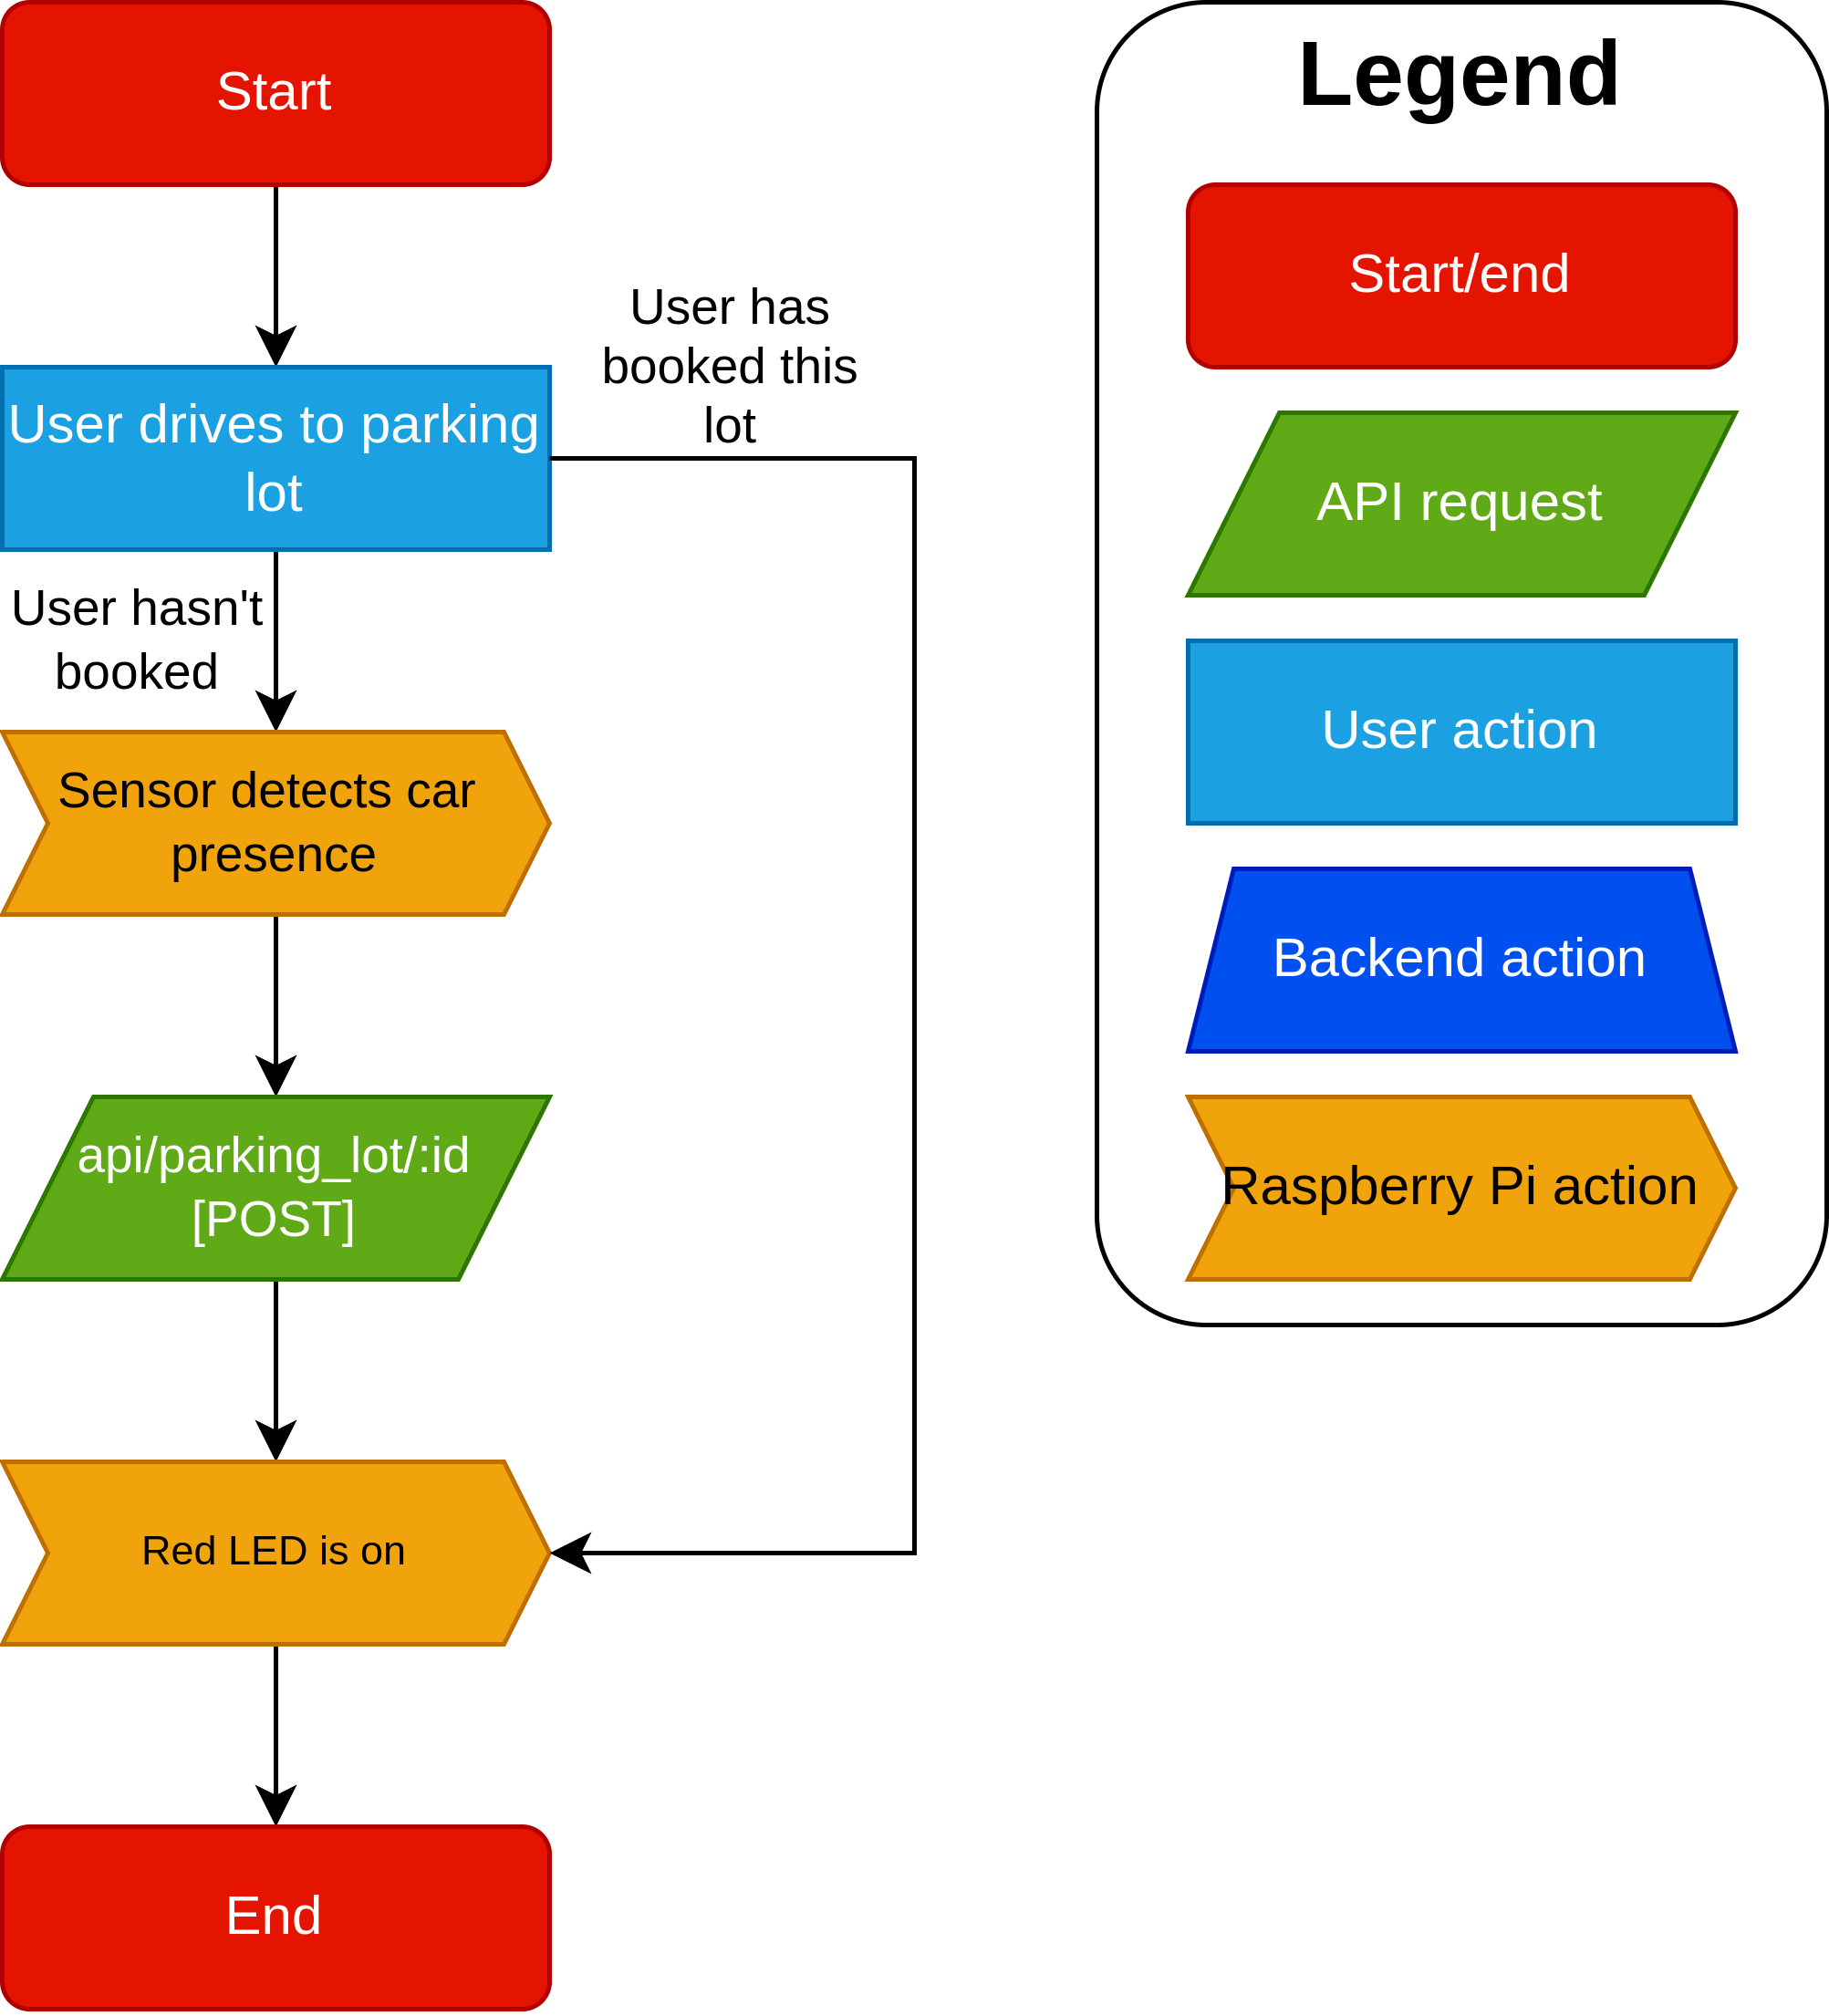
\includegraphics[width=7cm]{images/car_detection.drawio.png}
    \caption{Flowchart of the car detection process of the garage in both hardware, software and user terms.}
    \label{fig:car-detection}
\end{figure}

\begin{figure}[htp]
    \centering
    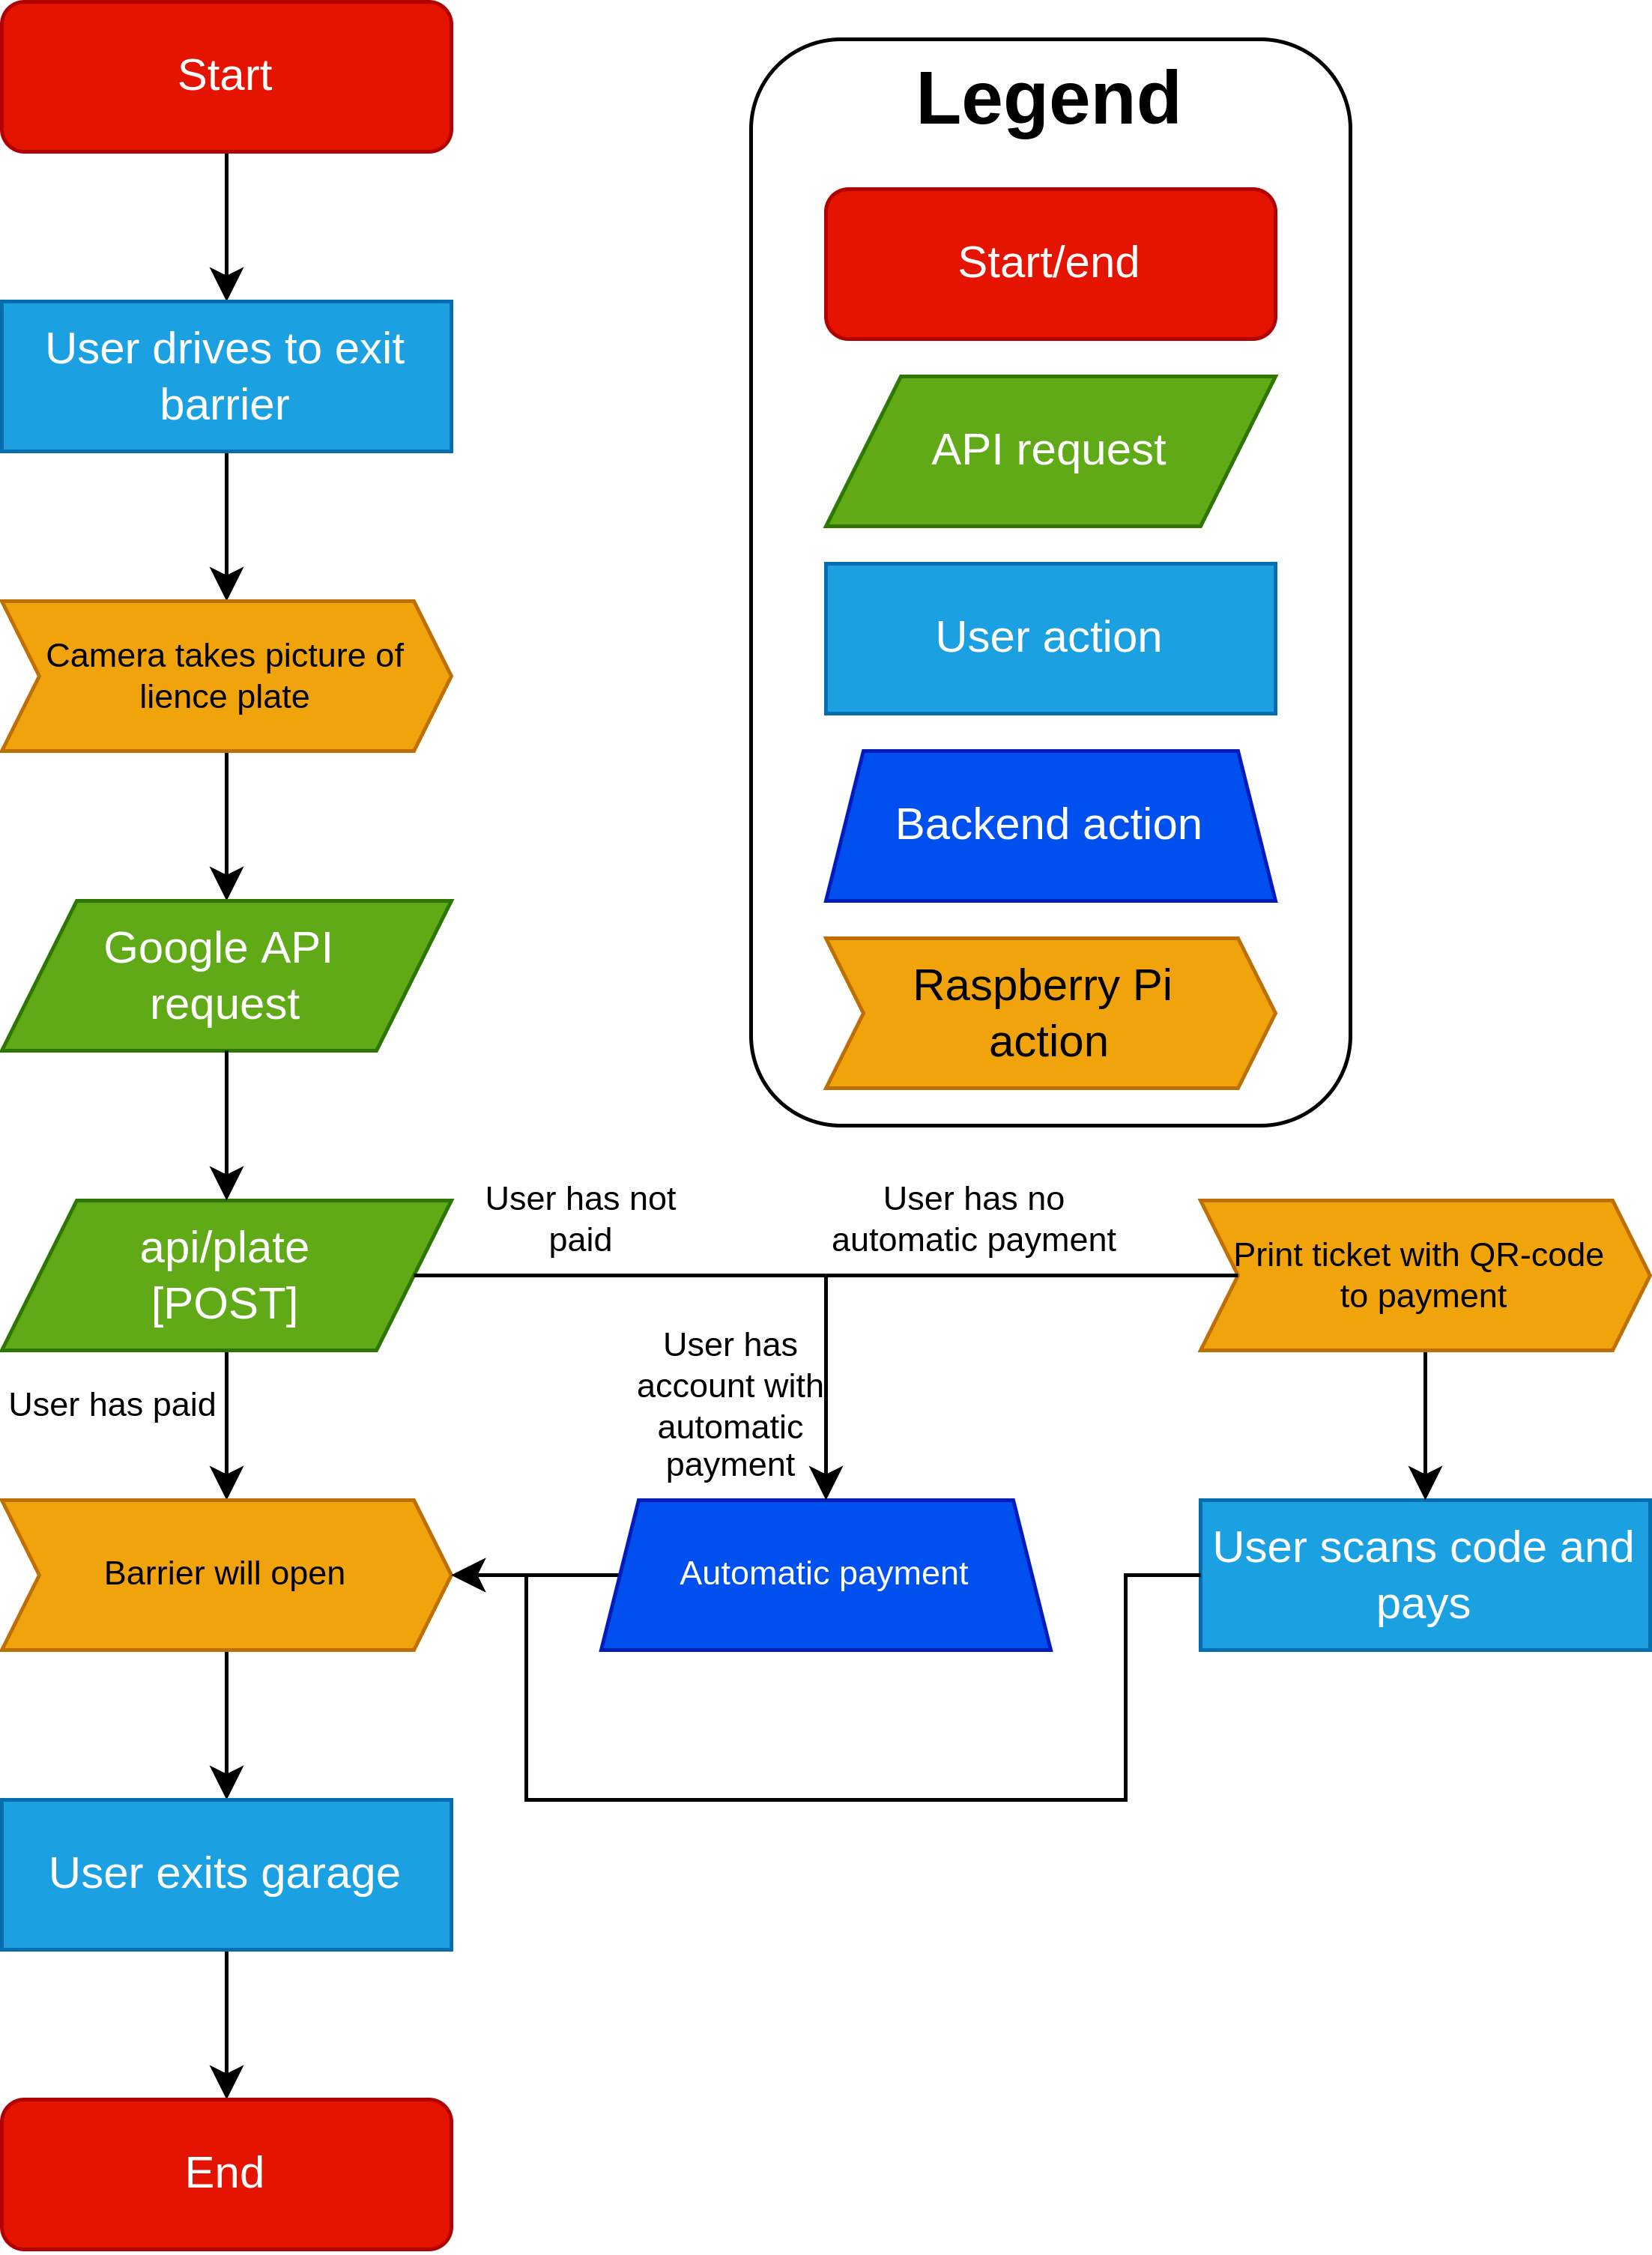
\includegraphics[width=8cm]{images/garage_exit.drawio.png}
    \caption{Flowchart of the exiting process of the garage in both hardware, software and user terms.}
    \label{fig:garage-exit}
\end{figure}

\section{Sequence diagrams}\label{app:sequence-diagrams}
\begin{figure}
    \centering
    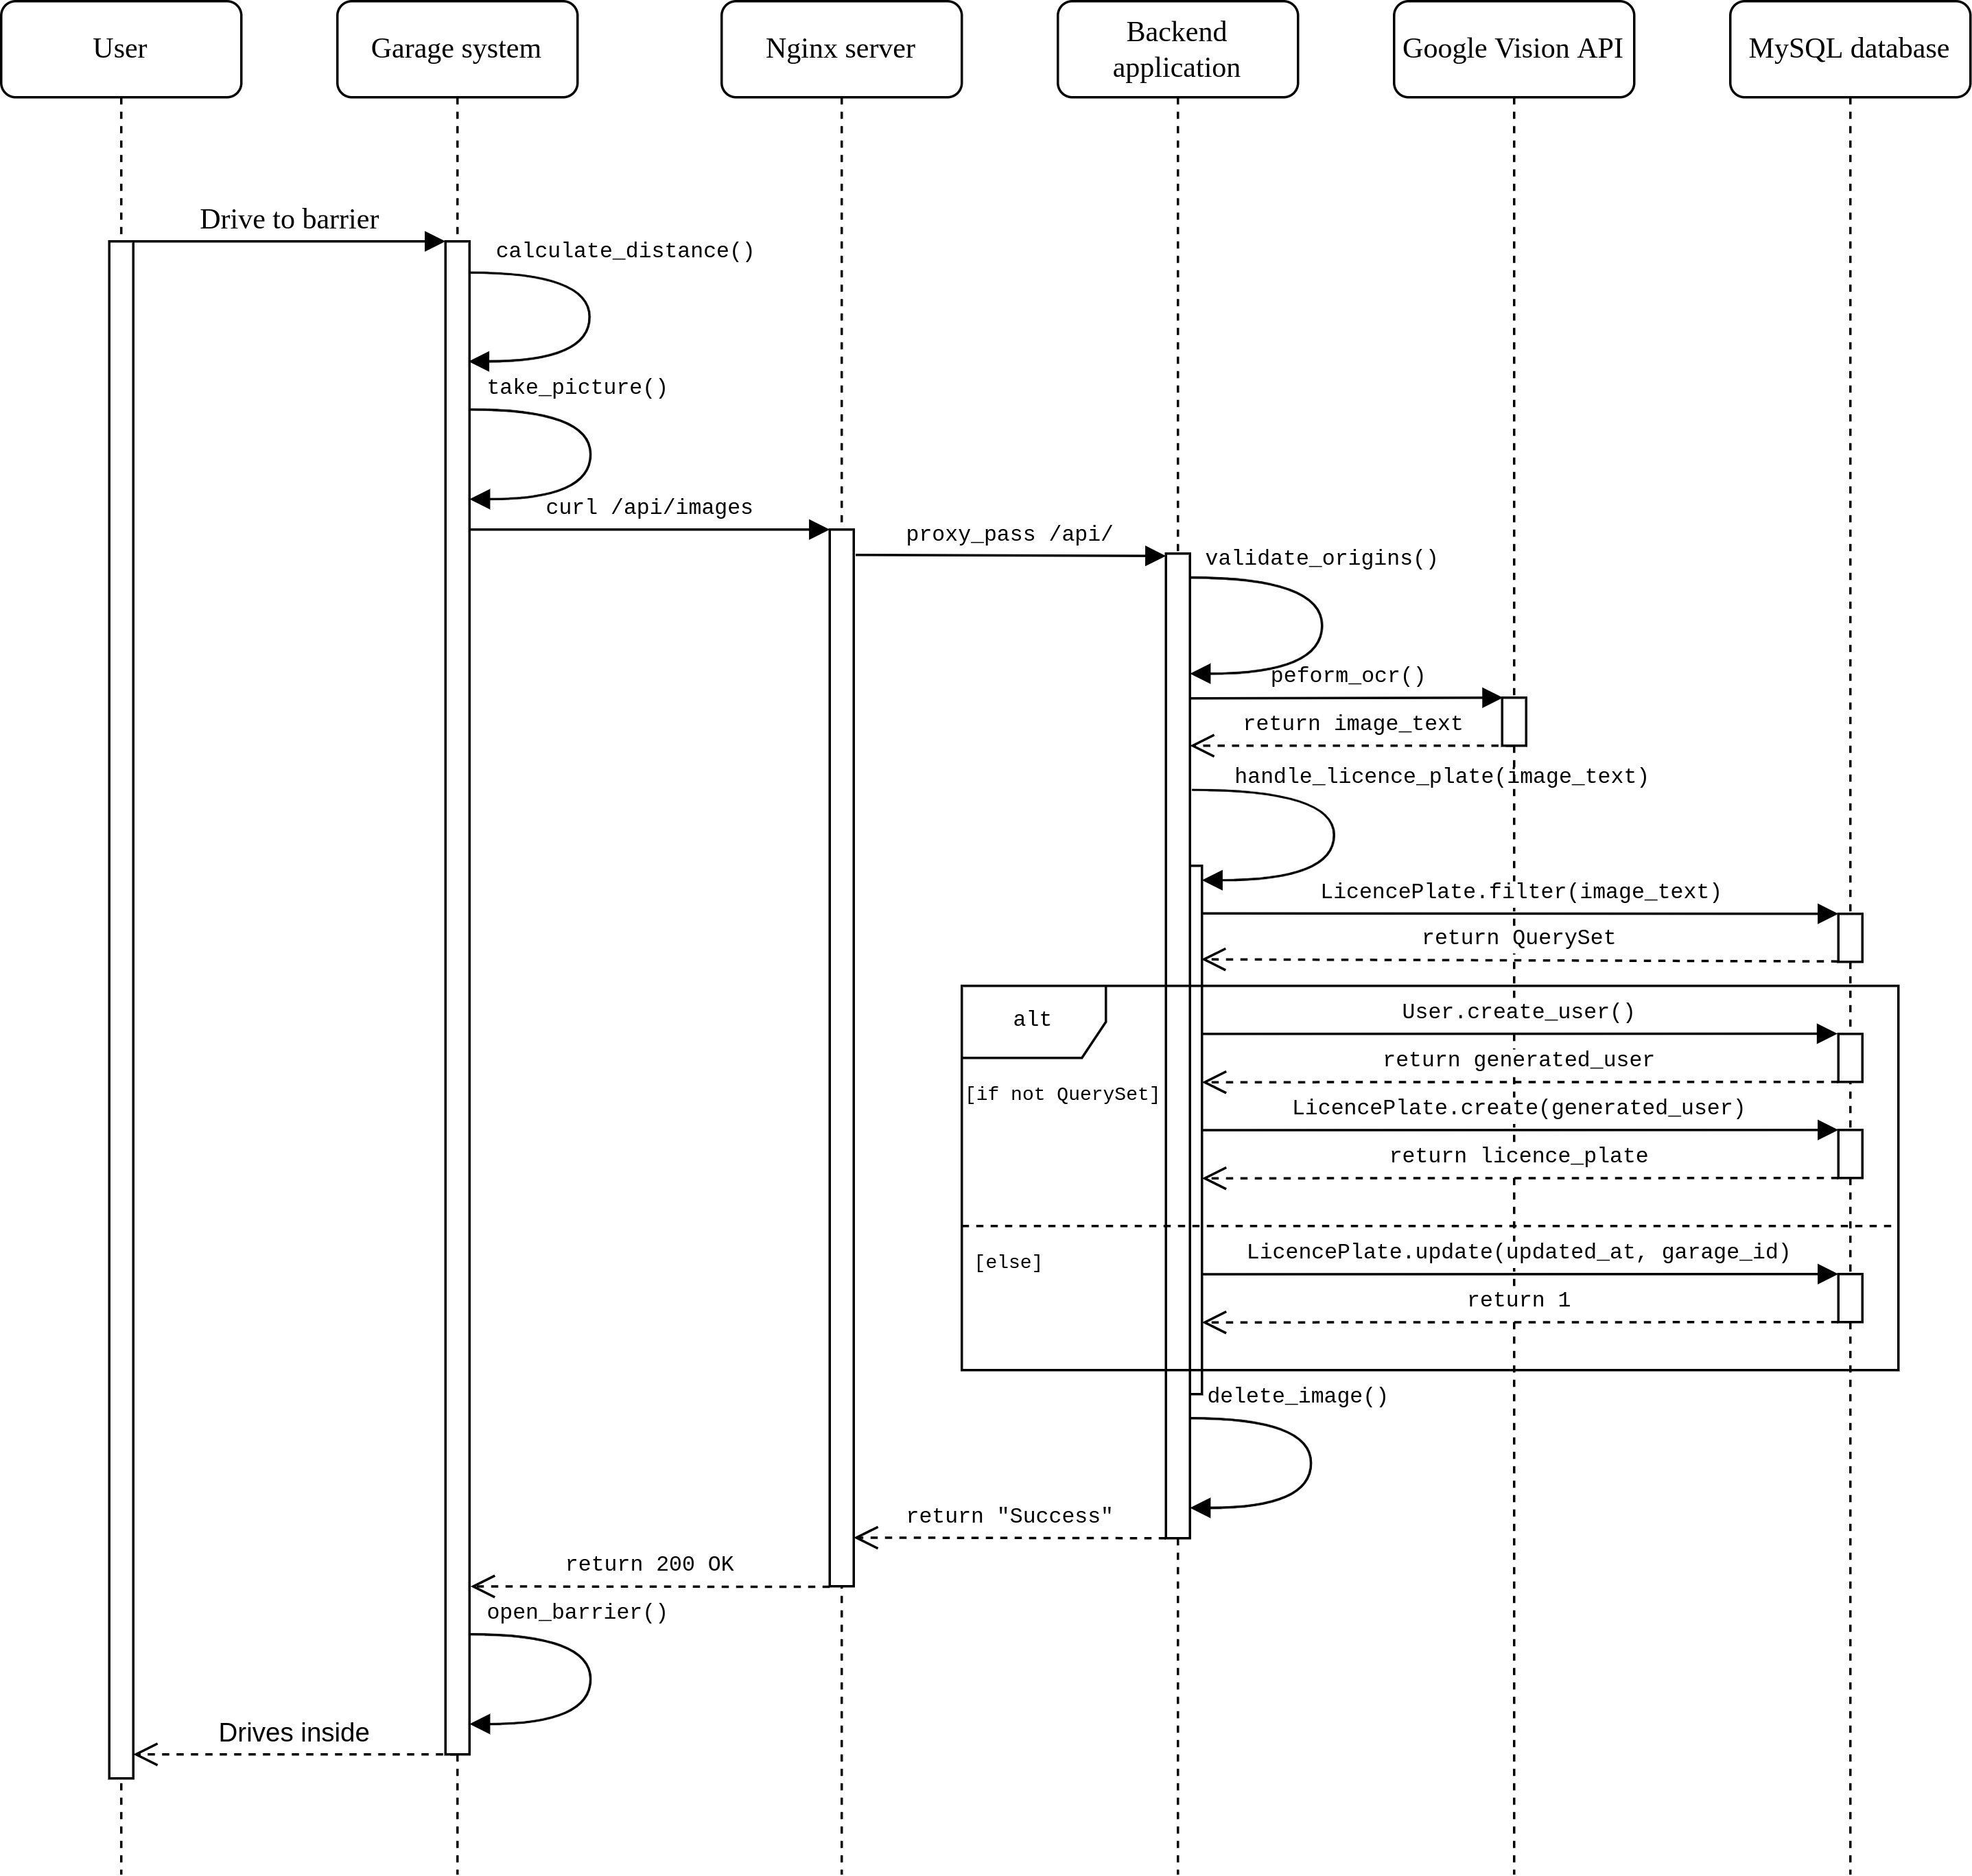
\includegraphics[width=16cm]{images/sequence_diagram_licence_plate.drawio.png}
    \caption{Sequence diagram of the licence plate registration in the local garage system.}
    \label{fig:sequence-diagram-licence-plate}
\end{figure}

\begin{figure}
    \centering
    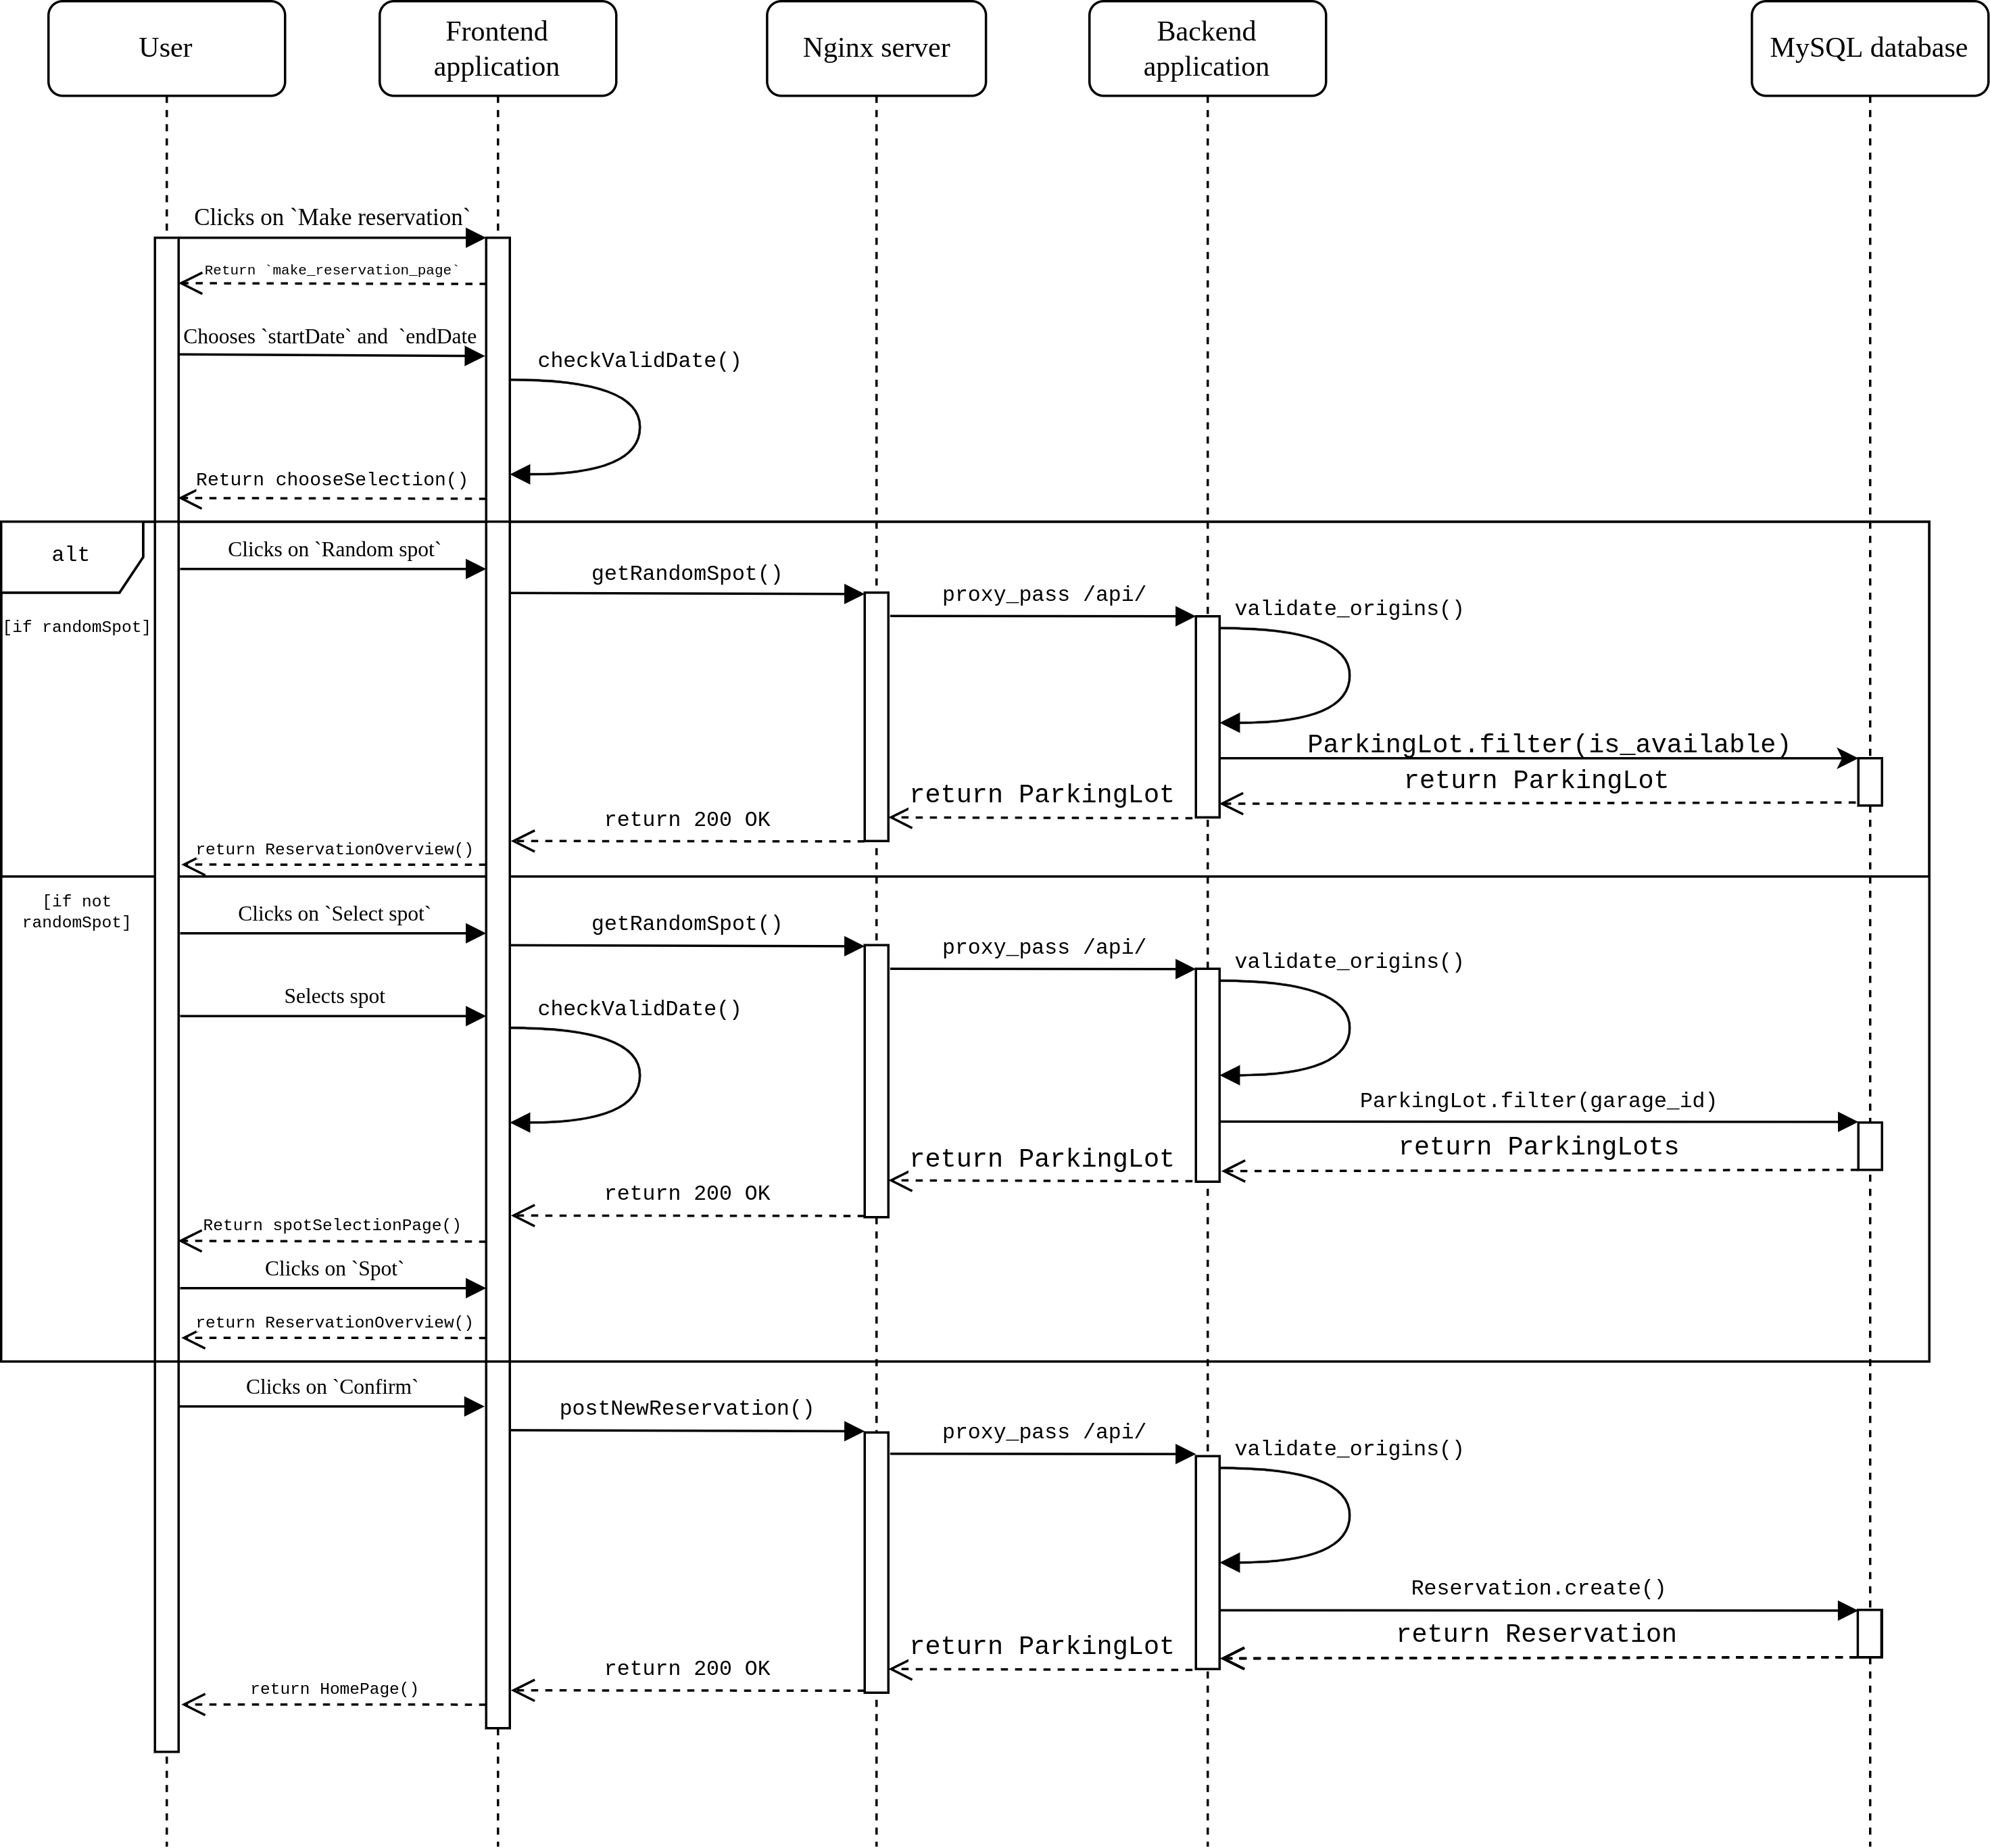
\includegraphics[width=16cm]{images/sequence_diagram_reservation.drawio.png}
    \caption{Sequence diagram of the reservation flow.}
    \label{fig:sequence-diagram-reservation}
\end{figure}
\end{comment}
\end{appendices}
